\graphicspath{{./figures/}}

\section{Overview}

The requirements for this project are defined by analysing general, currently existing balloon-satellite systems, as well as taking into account the planned launch that this specific \mbox{PocketQube} will be used in, as shown in Figure \ref{fig:balloon_path}. Further, the desired integration with the existing Radiosonde system (the iMet-54 device) is taken into account.

Generally, high-altitude balloons can drift to a height as much as 30 km above sea level \cite{site-weatherWeatherBalloons}. For this project, the balloon is planned to be released from near Saldanha Bay (Western Cape, South Africa), where it will travel a maximum distance of around 200 km towards the Cederberg and land furthest in Worcester. From Cape Town, this is a maximum straight line distance of around 115 km. 

\begin{figure}[!htb]
  \centering
  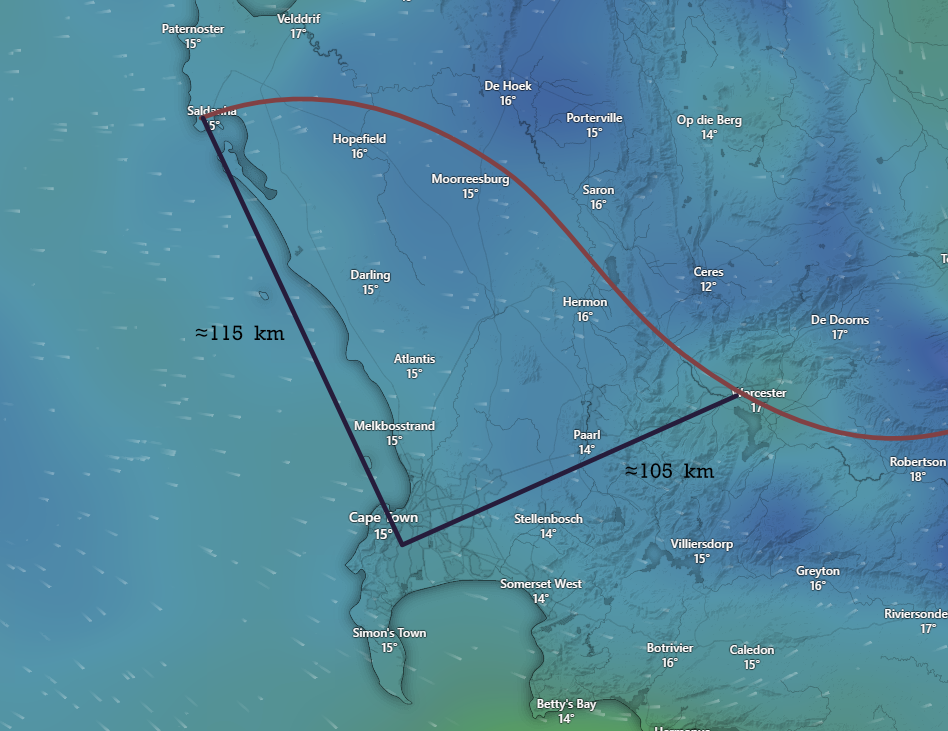
\includegraphics[width=0.8\textwidth]{balloon_path}
  \caption{Balloon Path and Distances}
  \label{fig:balloon_path}
\end{figure}